\documentclass[paper=a4]{jlreq}
\usepackage{amsmath,amssymb}
\usepackage{here}
\usepackage{graphicx}
\usepackage{hyperref}
\usepackage{physics}
\usepackage{subcaption}
\usepackage{tikz}
\usepackage{xcolor}

\definecolor{cud_red}{cmyk}{0,0.75,0.9,0}
\definecolor{cud_green}{cmyk}{0.75,0,0.65,0}
\definecolor{cud_blue}{cmyk}{1,0.45,0,0}

\hypersetup{
    colorlinks=true,
    linkcolor=cud_blue,
    citecolor=cud_green,
    filecolor=cud_blue,      
    urlcolor=cud_green,
}

\usetikzlibrary{intersections, calc, arrows}

\begin{document}
\title{FEMで1次元Poisson方程式を解く}
\author{きゅーしす}
\maketitle

\section{はじめに}

有限要素法(Finite Element Method)
は微分方程式の数値解法の一つで, 構造解析などの様々な問題に適用されている.
有限要素法は微分方程式を領域を要素の集まりに分割し, 
それぞれの要素内部で補間関数で近似する.
有限要素法は以下の手順で問題を解く.
\begin{enumerate}
    \item 領域を要素の集まりに分割する
    \item 微分方程式を積分して弱形式を求める
    \item 要素ごとに積分して離散化する
    \item 離散化した連立方程式を解く
\end{enumerate}

ここでは理解のために1次元Poisson方程式を有限要素法で解き, 結果をまとめる.

\section{有限要素法}
この節では有限要素法の概要を文献\cite{nakajima}を参考に説明し, 
有限要素法を1次元Poisson方程式に適用して離散化を行い, 連立方程式を得る.

\subsection{1次元Poisson方程式}
1次元の領域$\Omega$において1次元のPoisson方程式成り立つものとする. 
ここで, $q$は定数とする.
\begin{align}
    \dv[2]{u}{x} + q = 0 \quad x \in \Omega \label{eq:poisson}
\end{align}


\subsection{要素の分割と補間関数による近似}
有限要素法では領域を分割し, 要素ごとに近似関数で補間を行って解を表現する.
近似関数は形状関数と呼ばれ, 多項式関数である.形状関数が$p$次の要素を$p$次要素という.
今回は最も簡単な1次要素を用いる.要素の幅は不均等である.
図\ref{fig:decompose}に領域を要素に分割した様子を示す.
ただし, $k$番目の接点番号, 要素番号, 要素の幅をそれぞれ
$k,\quad (k), \quad l^{(k)}$とした.
\begin{figure}[htbp]
    \centering
    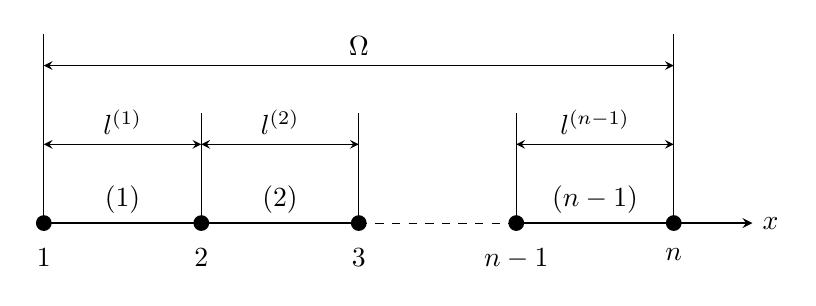
\begin{tikzpicture}[x=2cm,y=2cm]
        %x軸
        \draw[semithick] (0,0)--(2,0);
        \draw[dashed] (2,0)--(3,0);
        \draw[->,>=stealth,semithick] (3,0)--(4.5,0)node[right]{$x$};

        \foreach \x in {0,...,4} \fill[black](\x,0) circle (0.1/2); %接点の円
        %接点の番号
        \foreach \x in {1,...,3} \draw (\x-1,-0.1)node[below]{\x};
        \draw (3,-0.1)node[below]{$n-1$} (4,-0.1)node[below]{$n$};
        %領域\Omega
        \draw (0,0)--(0,1.2) (4,0)--(4,1.2);
        \draw[<->,>=stealth] (0,1)--(2,1)node[above]{$\Omega$}--(4,1);
        %要素の長さ
        \foreach \x in {1,...,3} \draw (\x,0)--(\x,0.7);
        \draw[<->,>=stealth] (0,0.5)--(0.5,0.5)node[above]{$l^{(1)}$}--(1,0.5);
        \draw[<->,>=stealth] (1,0.5)--(1.5,0.5)node[above]{$l^{(2)}$}--(2,0.5);
        \draw[<->,>=stealth] (3,0.5)--(3.5,0.5)node[above]{$l^{(n-1)}$}--(4,0.5);
        %要素番号
        \draw (0.5,0)node[above]{$(1)$} (1.5,0)node[above]{$(2)$};
        \draw (3.5,0)node[above]{$(n-1)$};
    \end{tikzpicture}
    \caption{要素分割と接点配置}
    \label{fig:decompose}
\end{figure}

要素内部で補間に用いられる関数は形状関数と呼ばれ, 接点数と同じ数存在する.
形状関数は接点$i,j$に対して
以下の性質をもつ.
\begin{itemize}
    \item 接点$i$に対して形状関数$N_i(x_i) = 1$
    \item 接点$i$を除く全ての接点$j$にたいして$N_i(x_j) = 0$
\end{itemize}
1次要素に対して形状関数を求める.接点$i,j$をもつ要素$k$があり, 
$l^{(k)} = x_j-x_i$とすると形状関数$N_j,N_j$は
\begin{align}
    N_i(x) & = \frac{x_j -x}{l^{(k)}} \label{eq:shape:i}  \\
    N_j(x) & = -\frac{x_i -x}{l^{(k)}} \label{eq:shape:j}
\end{align}
となる.この形状関数をプロットしたものを図\ref{fig:shape_function}に示す.
要素内部で形状関数の線型結合で近似する.接点$i$の物理量を$u_i$とすると
以下の式となる.
\begin{align}
    u = u_iN_i+u_jN_j \label{eq:shape:linear-comb:scalar}
\end{align}
式\eqref{eq:shape:linear-comb:scalar}を図\ref{fig:interpolation}に示す.ベクトル
\begin{align}
    [N]   & = [N_i \quad N_j] \label{eq:shape:mat}           \\
    \{u\} & = [u_i \quad u_j]^\intercal \label{eq:value:mat}
\end{align}
を用いて表記すると式\eqref{eq:shape:linear-comb:scalar}は以下のようになる.
\begin{align}
    u = [N]\{u\} \label{eq:shape:linear-comb}
\end{align}

\begin{figure}[htbp]
    \centering
    \begin{subfigure}{0.49\columnwidth}
        \centering
        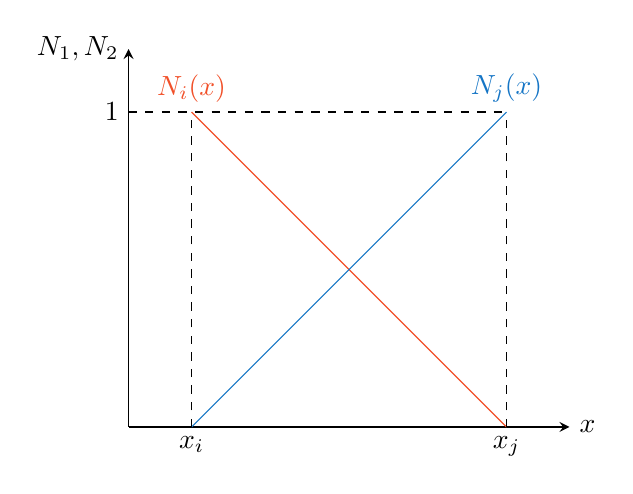
\begin{tikzpicture}[x=4cm,y=4cm]
            \draw[->,>=stealth,semithick] (0,0)--(1.4,0)node[right]{$x$}; %x軸
            \draw[->,>=stealth,semithick] (0,0)--(0,1.2)node[left]{$N_1,N_2$}; %y軸
            %形状関数
            \draw[cud_red](0.2,1)node[above]{$N_i(x)$}--(1.2,0);
            \draw[cud_blue](0.2,0)--(1.2,1)node[above]{$N_j(x)$};
            %点線とメモリ
            \draw[dashed] (0,1)node[left]{$1$}--(1.2,1);
            \draw[dashed] (0.2,0)node[below]{$x_i$}--(0.2,1);
            \draw[dashed] (1.2,0)node[below]{$x_{j}$}--(1.2,1);
        \end{tikzpicture}
        \caption{1次元1次要素の形状関数}
        \label{fig:shape_function}
    \end{subfigure}
    \begin{subfigure}{0.49\columnwidth}
        \centering
        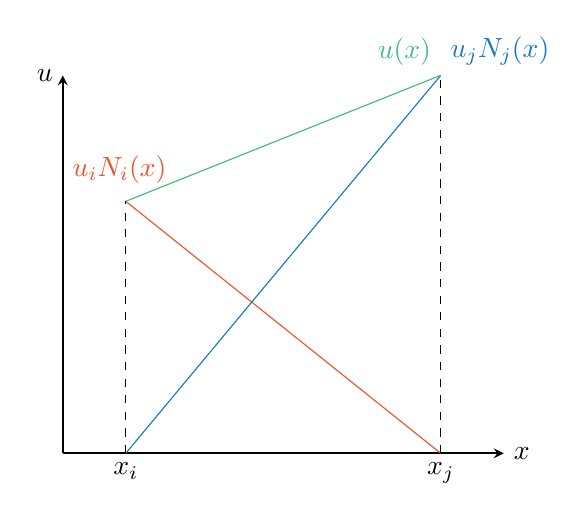
\begin{tikzpicture}[x=4cm,y=4cm]
            \draw[->,>=stealth,semithick] (0,0)--(1.4,0)node[right]{$x$}; %x軸
            \draw[->,>=stealth,semithick] (0,0)--(0,1.2)node[left]{$u$}; %y軸
            %形状関数
            \draw[cud_red](0.2,0.8)--(1.2,0);
            \draw[cud_red] (0,0.9)node[right]{$u_iN_i(x)$};
            \draw[cud_blue](0.2,0)--(1.2,1.2)node[above right]{$u_jN_j(x)$};
            \draw[cud_green](0.2,0.8)--(1.2,1.2)node[above left]{$u(x)$};
            %点線とメモリ
            \draw[dashed] (0.2,0)node[below]{$x_i$}--(0.2,0.8);
            \draw[dashed] (1.2,0)node[below]{$x_{j}$}--(1.2,1.2);
        \end{tikzpicture}
        \caption{形状関数を用いた補間}
        \label{fig:interpolation}
    \end{subfigure}
    \caption{形状関数による補間}
\end{figure}


\subsection{弱形式}
積分して弱形式を求める手法はいくつかあるが, 今回は重み付き残差法を用いる.
重み付き残差法は対象とする微分方程式に重み関数を掛けて積分することで離散化する.
今回, 1次元のPoisson方程式\eqref{eq:poisson}を重み付き残差法で離散化する.
解を近似したときの誤差を残差といい以下の式で与えられる.
\begin{align}
    R = \dv[2]{u}{x} +q    \label{eq:residal}
\end{align}
重み付き残差法では以下に示す残渣に重み関数を乗じて要素全体の残差を0とする条件を与える.
このとき, 解は一意に定まる.ここで要素$e$の領域を$\Omega^{(e)}$とする.
\begin{align}
    \int_{\Omega^{(e)}} wR\dd{x} = \int_{\Omega^{(e)}} w\qty( \dv[2]{u}{x} + q)\dd{x} = 0\quad
    \text{for all}\,w
    \label{eq:weighted-residual}
\end{align}
重み関数はいくつかの定義があるが, 
今回は重み関数が形状関数と等しいGalerkin法を適用する.
ここで形状関数(式\eqref{eq:shape:mat})を代入して
\begin{align}
    \int_{\Omega^{(e)}} [N]^\intercal \dv[2]{u}{x}\dd{x}
    + \int_{\Omega^{(e)}} [N]^\intercal q\dd{x} & = \vb*{0} \label{eq:galerkin}
\end{align}
となるが左辺第1項が常に0となり, 
解が一意に定まらないので2階微分を1階微分にする必要がある.
したがって以下の部分積分の公式を用いて1階微分の積で表す.
\begin{align}
    \int_{\Omega^{(e)}} \qty(\phi\dv[2]{\psi}{x}) \dd{x} &=
    \eval{\qty(\phi\dv{\psi}{x})}_{\Gamma^{(k)}}
    - \int_{\Omega^{(e)}} \qty(\dv{\phi}{x}\dv{\psi}{x}) \dd{x}
    \label{eq:gauss-green:theorem}
\end{align}

式\eqref{eq:galerkin}に代入して計算すると以下のようになり, 式を得る.ただし, $J=-\dv*{u}{x}$とし, 
$\Gamma^{(k)}$は領域$\Omega^{(k)}$の両端の境界とする.
\begin{align}
    \eval{\qty([N]^\intercal\dv{u}{x})}_{x_i}^{x_j}
    - \int_{\Omega^{(e)}} \dv{[N]^\intercal}{x} \dv{u}{x}\dd{x}
    + \int_{\Omega^{(e)}} [N]^\intercal q\dd{x} & = \vb*{0} \notag               \\
    -\eval{\qty([N]^\intercal J)}_{x_i}^{x_j}
    - \qty(\int_{\Omega^{(e)}} \dv{[N]^\intercal}{x} \dv{[N]}{x}\dd{x})\cdot\{u\}
    + \int_{\Omega^{(e)}} [N]^\intercal q\dd{x} & = \vb*{0} \label{eq:weak_form}
\end{align}
式\eqref{eq:weak_form}を弱形式といい, 支配方程式(式\eqref{eq:poisson})に対応する.
次に, 要素$e$の弱形式をマトリクス形式で表記する.以下のマトリクス
\begin{align}
    [k]^{(e)}   & = \int_{\Omega^{(e)}} \dv{[N]^\intercal}{x} \dv{[N]}{x}\dd{x}  \label{eq:local_matrix}                        \\
    \{f\}^{(e)} & = \int_{\Omega^{(e)}} [N]^\intercal q\dd{x} - \eval{\qty([N]^\intercal J)}_{x_i}^{x_j}\label{eq:local_vector}
\end{align}
を用いて以下のマトリクス形式の弱形式を得る.
\begin{align}
    [k]^{(e)}\{u\}^{(e)} =  \{f\}^{(e)}
    \label{eq:weak_form:mat}
\end{align}
形状関数は式\eqref{eq:shape:i}, \eqref{eq:shape:j}であるので
以下のマトリクス形式の形状関数とその導関数を得る.
\begin{align}
    [N]         & =
    \begin{bmatrix}
        \frac{x_j -x}{l^{(e)}} &
        \frac{x - x_i}{l^{(e)}}
    \end{bmatrix} \\
    \dv{[N]}{x} & =
    \begin{bmatrix}
        -\frac{1}{l^{(e)}} &
        \frac{1}{l^{(e)}}
    \end{bmatrix}
\end{align}
これを$[k]^{(e)}$に代入して計算する.
\begin{align}
    [k]^{(e)} & =
    \begin{bmatrix}
        -\frac{1}{l^{(e)}} \\
        \frac{1}{l^{(e)}}
    \end{bmatrix}
    \begin{bmatrix}
        -\frac{1}{l^{(e)}} &
        \frac{1}{l^{(e)}}
    \end{bmatrix}
    \int_{\Omega^{(e)}}\dd{x}
    = \frac{1}{l^{(e)}}
    \begin{bmatrix}
        1  & -1 \\
        -1 & 1
    \end{bmatrix}
\end{align}
次に$\{f\}^{(e)}$を計算する.
要素の重なり合う場所で打ち消されるので, 第1項は領域境界の要素のみ残る.
第二項のみ計算して
\begin{align}
    \{f\}^{(e)} = \frac{ql^{(e)}}{2}
    \begin{bmatrix}
        1 \\
        1
    \end{bmatrix}
\end{align}
これら要素単位での計算ができた.

\subsection{全体マトリクスとベクトル}
要素ごとに計算した結果から全体マトリクスを生成する.
要素$e_1$の局所節点番号が$i$が全体節点番号$j$になり,
一つの要素$e_2$の局所節点番号が$k$が全体節点番号$j$になるとき,
全体節点ベクトル$\{F\}$の$j$番目の行$\{F\}_j$は
\begin{align}
    \{F\}_j = \{f\}^{(e_1)}_i +  \{f\}^{(e_2)}_k 
\end{align}
となる. アルゴリズムにまとめると以下のようになる. 

\subsection{境界条件の適用}
境界条件のおもなものにDirichlet条件とNeumann条件の2種類がある.
Dirichlet条件は一部の節点において解が設定されている条件で境界条件が直接代入できる.
一方でNeumann条件は微分値となるので未知数となる. 

節点$i$にDirichlet 条件$u_D$を課すことを考える.
節点$i$については$u_i =u_D$が成立する. 先ほど求めた全体マトリクスに対してこれを適用すると,
マトリクス$[K]$の$i$行について対角成分を1とし, それ以外の成分を0とする.
このままではマトリクス$[K]$が非対称な行列となり連立方程式の解法で不都合が生じることがあるので
$[K]$の対称性を保つために$i$列の項を移項して行列$[K]$の対称性を維持する.
$i$列の$i$行以外の成分を移項する. 
$j$を$i$でない数として全体ベクトルの$j$行から$[K]_{ji}u_D$を差し引く.

Neumann 条件は微分値を指定しており, 
未知数となるので式\eqref{eq:local_vector}を要素マトリクスを計算するときに
Neumann条件を計算して代入する.

\section{計算例}
前述した手法を検証するべく, 境界値問題を解く.
今回解く1次元Poisson方程式の境界値問題は
\begin{align}
    \begin{aligned}
        \dv[2]{u}{x}       + 2 & = 0 \quad \mathrm{for}\quad (0 \leq x \leq 1) \\
        u|_{x=1}               & = 1                                        \\
        \eval{\dv{u}{x}}_{x=0} & = 2
    \end{aligned}
    \label{eq:poisson_example}
\end{align}
とする. 解析解は以下の式で表される.
\begin{align}
    u(x) = -x^2+2x
\end{align}
要素数は5つとし, それぞれの幅0.2とした. 
結果を図\ref{fig:result}に示す. FEMと解析解が一致していることが確認できる.
\begin{figure}[htbp]
    \centering
    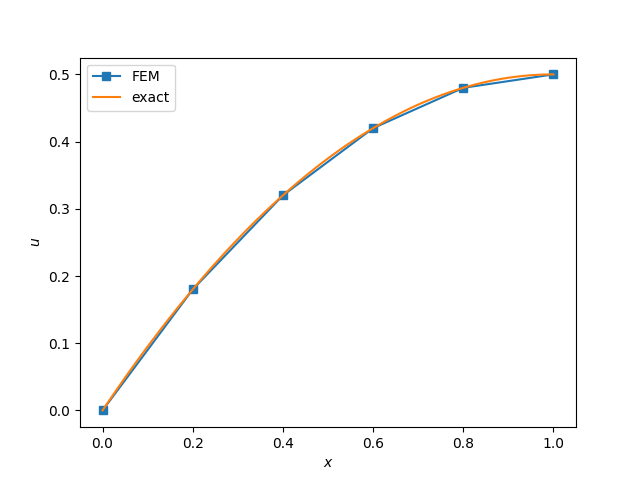
\includegraphics[width=10cm]{5-elements.png}
    \caption{FEMの計算結果と解析解}
    \label{fig:result}
\end{figure}

\begin{thebibliography}{9}
    \bibitem{nakajima}
    中島研吾,
    有限要素法による一次元定常熱伝導解析プログラム C言語編,
    \url{http://nkl.cc.u-tokyo.ac.jp/FEM/02-FEM1D-C.pdf} \today 閲覧
\end{thebibliography}

\end{document}